\documentclass{article}
\usepackage{pgfplots}
\pgfplotsset{compat=newest}
\begin{document}
\pgfplotsset{footnotesize,samples=10, domain=0:1,point meta min=0, point meta max=1}
\begin{center}% note that \centering uses less vspace...
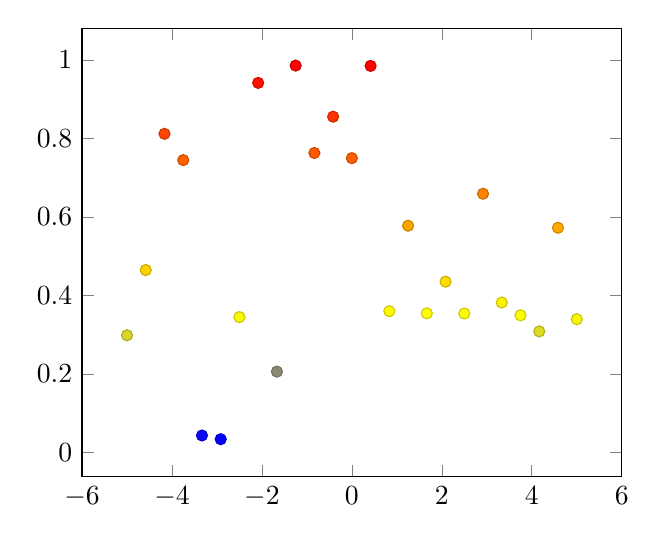
\begin{tikzpicture}
	\begin{axis}[colorbar,colorbar horizontal,colorbar to name={storedcolorbar}]
	\addplot[scatter,only marks,mark=*] {rnd};
	\end{axis}
\end{tikzpicture}
%
\begin{tikzpicture}
	\begin{axis}
	\addplot+[domain=0:1,mark=none,mesh] {x^2};
	\end{axis}
\end{tikzpicture}
%
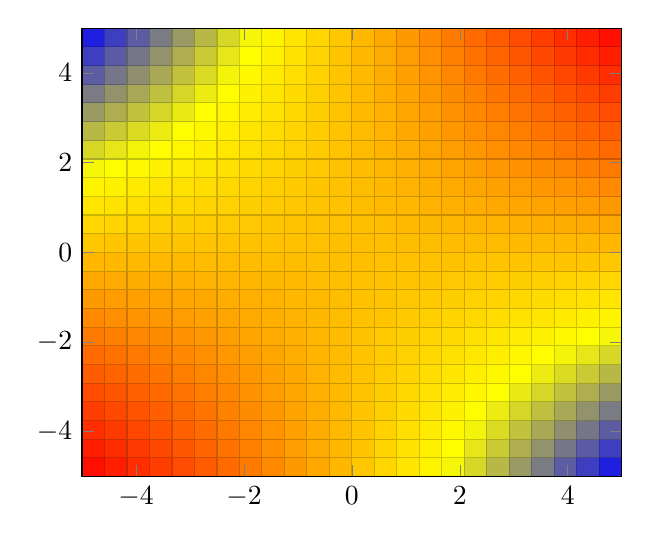
\begin{tikzpicture}
	\begin{axis}[view={0}{90}]
	\addplot3[surf] {x*y};
	\end{axis}
\end{tikzpicture}
\\
\ref{storedcolorbar}
\end{center}
\end{document}
